\documentclass[conference]{IEEEtran}
% \documentclass[journal,peerreview]{IEEEtran}


\usepackage[dvips]{graphicx}
% *** MATH PACKAGES ***
%
\usepackage[cmex10]{amsmath}
% Also, note that the amsmath package sets \interdisplaylinepenalty to 10000
% thus preventing page breaks from occurring within multiline equations. Use:
\interdisplaylinepenalty=2500
%
\usepackage{amsfonts}
\usepackage{amssymb}
\usepackage{spconf}
\usepackage{float}


\usepackage[caption=false,font=footnotesize]{subfig}

% *** PDF, URL AND HYPERLINK PACKAGES ***
%
\usepackage{url}


\usepackage[nolist]{acronym}
\usepackage{paralist}
\usepackage{tikz} % Create graphics in Latex
\usetikzlibrary{positioning}
\usetikzlibrary{fit}

% correct bad hyphenation here
\hyphenation{op-tical net-works semi-conduc-tor}

%\renewcommand{\baselinestretch}{0.999}
%
%\ninept

\begin{document}
	
	%\abovedisplayskip=.7\belowdisplayskip
%	\belowdisplayskip=.7\belowdisplayskip
	
	\title{Estimation of Multivariate Probability density function using the maximum entropy principle}
	
	%\ifCLASSOPTIONpeerreview
	%\author{Author~1,
	%        Author~2,
	%        Author~3
	%}
	%\else
	\twoauthors{Zois Boukouvalas}{ department. \\American University \\ Washington DC, USA \\ boukouva@american.edu}{Charles C. Cavalcante, Lucas P. Damasceno}{ department. \\ Federal University of Ceará\\ Fortaleza, 60455-760 Brazil \\ charles@gtel.ufc.br \\ lucaspdamasceno@alu.ufc.br}
	
	%\fi
	%\ifCLASSOPTIONpeerreview
	%\author{Author~1,
	%        Author~2,
	%        Author~3
	%}
	%\else
	%\author{Author~1,
	%        Author~2,
	%        Author~3
	%}
	%\fi
	
	
	
	
	% make the title area
	\maketitle
	
	% As a general rule, do not put math, special symbols or citations
	% in the abstract or keywords.
\begin{abstract}
%
The estimation of a multivariate probability density function is a fundamental problem in statistics and estimation theory. In this paper, we use the maximum entropy principle as a versatile tool with specified constraints, also we employ both global and local measuring functions, where Gaussian kernels are used as local measuring functions. Here, we present a computational framework for a multivariate density estimator with a convex optimization algorithm based on the Newton method and Monte Carlo multidimensional integration method. Experimental results are based on a two-dimensional space and can be extended to higher-dimensional. Our numerical results demonstrate rapid convergence and consistent trends with the proposed theory.
\end{abstract}
	
% Note that keywords are not normally used for peerreview papers.
%\begin{IEEEkeywords}
%Precoder selection, message passing, distributed optimization.
%\end{IEEEkeywords}
	
	
\begin{IEEEkeywords}
	Multivariate probability density estimation, Maximum entropy distributions, Gaussian Kernel, Monte Carlo methods.
\end{IEEEkeywords}
	
	
	% For peer review papers, you can put extra information on the cover
	% page as needed:
	% \ifCLASSOPTIONpeerreview
	% \begin{center} \bfseries EDICS Category: 3-BBND \end{center}
	% \fi
	%
	% For peerreview papers, this IEEEtran command inserts a page break and
	% creates the second title. It will be ignored for other modes.
	%\IEEEpeerreviewmaketitle
	
\section{Introduction}
	
The estimation of a multivariate probability density function (PDF) is a common problem in a wide variety of fields, ranging from physics to statistics. Within the field of Artificial Intelligence (AI) and its subfields deep learning, machine learning, and computer vision require knowledge of the data’s PDF either explicitly or implicitly. Therefore, effective density characterization is vital to the success of these AI approaches.
%
	
Multidimensional density estimation approaches can be broadly classified into two groups, parametric multidimensional methods, and non-parametric multidimensional methods. The parametric multidimensional methods, such as the multivariate generalized Gaussian distribution (GGD) \cite{sara:2005} and the multivariate maximum likelihood estimation, use prior assumptions about the form of the underlying density function. Such assumptions simplify the problem since only the parameters of the chosen family of functions need to be determined. In most problems, it is not possible to assume anything about the form of the underlying density function. Thus, non-parametric multidimensional methods, such as histogram estimation, k-nearest neighbors, and kernel density estimation, are more appropriate in these situations, since these techniques make few assumptions about the density function and allow the data to drive the estimation process more directly.
%
	
In this paper, we present a multivariate density estimator with smooth characteristics based on the maximum entropy principle. We jointly use global and local measuring functions to provide flexible PDFs with as simple a form as possible. The global measuring functions yield constraints on the statistics of the PDF, such as the mean, variance, and higher-order statistics (HOS). However, methods using only global measuring functions ignore local information, i.e., characteristics in a given interval, of the PDF, additionally, the use of higher-order polynomials can introduce stability issues. We use Gaussian kernels, which do not have stability issues due to their localized characteristics, as local measuring functions to provide local information. We call the new estimator multivariate entropy maximization with kernels (M-EMK) and consider it as an extension of the univariate case \cite{Zois:2015}.
	
%
	
\section{ Background }
\label{sec:sys_model}
The maximum entropy principle states that the probability distribution which best represents the current state of knowledge is the one with the largest entropy. Thus, the maximum entropy density, subject to known constraints, can be written as the following optimization problem \cite{Cover2006}:
%

\begin{equation}
\begin{split}
\max_{{p(\mathbf{x})}}  H(p(\mathbf{x})) & = - \int_{-\infty}^{\infty} p(\mathbf{x})\log(\mathbf{x})d \mathbf{x} \\
\text{ s.t. } \int_{-\infty}^{\infty} r_i p(\mathbf{x}) d \mathbf{x} &= \alpha_i,
\text{ for }  i = 0,...,M,
\end{split}
\end{equation}
%
where $p(\mathbf{x})$ $\geq$ 0,  with equality outside the support set $\Omega(\mathbf{x})$, $r_i(\mathbf{x})\in C(\mathbb{R}^{K},\mathbb{R})$, $\forall i$, $C(\mathbb{R}^{K},\mathbb{R})$ represents the space of measuring functions which have domain $\mathbb{R}^{K}$ and codomain $\mathbb{R}$, and $\alpha_i = \sum_{t=1}^{T}  r_i(\mathbf{x_t})/T$ for $i = 0,...,M$ represents their corresponding sample averages, given observations $\mathbf{x}(t) \in \mathbb{R}^{K}$, $t = 1,...,T$. Therefore, $p$ is a density on support set $\Omega(\mathbf{x})$ meeting $M + 1$ constraints $\alpha_i,...,\alpha_M+1$. We note that the first constraint need to be $\int_{\Omega(\mathbf{x})} p(\mathbf{x}) d \mathbf{x} = 1$, equivalently $r_0 = 1$ and $\alpha_0 = 1$, in order for $p(\mathbf{x})$ to be a valid PDF.  The optimization problem in (1) can be rewritten as a Lagrangian function:
%
\begin{equation}
\mathcal{L}(p) = \int p\log p + \int p - 1 + \sum_{i=1}^{M}\lambda_i + \int r_i p - \alpha_i ,
\end{equation}
%	
where  $\lambda_i, i = 0,...,M$,  are the Lagrangian multipliers. Through the use of functional variation, we can “differentiate” (2) with respect to $p$. By setting $\partial\mathcal{L}(p)/\partial p = 0$, we obtain the equation of maximum entropy distribution,
%
\begin{equation}
p(\mathbf{x}) = \exp\left\{-1 + \sum_{i=0}^{M}\lambda_i r_i\left(\mathbf{x}\right)\right\},
\end{equation}
%
where Lagrangian multipliers are chosen such that $p$ satisfies the constraints in (1). By substituting (3) into the constraints in (1), we generate a nonlinear system of $M + 1$ equations for the $M + 1$ Lagrange multipliers. 

\section{M-EMK}
\subsection{Mathematical formulations} 
We can solve the equation (3) by the following Newton iteration,
%
\begin{equation}
\boldsymbol{\lambda}_{t+1} = \boldsymbol{\lambda}_{t} - \mathbf{J}^{-1} E_{p_{t}} \left\{\boldsymbol r - \boldsymbol\alpha\right\},
\end{equation}
%
where $p_t$ is the estimated PDF for the $t$th iteration, and        $\mathbf{r}=[r_0,...,r_M]$, $\boldsymbol{\lambda}=[\lambda_0,...,\lambda_M]$, $\boldsymbol{\alpha}=[\alpha_0,...,\alpha_M] \in \mathbb{R}^{M+1}$, and $\mathbf{J} \in \mathbb{R}^{M\times{M}}$, denote the vector of measuring functions, Lagrange multipliers, sample averages, and Jacobian matrix, respectively. The $ij$th entry of $\mathbf{J}$ is given by
%
\begin{equation} 
\begin{split}
 \mathbf{J}_{ij} &= \frac{\partial\int_{\Omega(\mathbf{x})} r_i(\mathbf{x}) p(\mathbf{x}) d \mathbf{x} - \alpha_i}{\partial\lambda_{j}} \\
 &= \int_{\Omega(\mathbf{x})} \frac{\partial p(\mathbf{x})}{\partial\lambda_{j}}  d \mathbf{x} \\
 &= \int_{\Omega(\mathbf{x})} r_i(\mathbf{x}) r_j(\mathbf{x}) p(\mathbf{x}) d \mathbf{x} \\
 &= E_{p_{t}}\left\{r_ir_j\right\},  \\
\end{split}
\end{equation}
%
and the  $i$th entry of $E_{p_{t}} \left\{\boldsymbol{r} - \boldsymbol\alpha\right\}$ is
%
\begin{equation}
E_{p_{t}} \left\{\boldsymbol{r} - \boldsymbol\alpha\right\}= \int_{\Omega(\mathbf{x})} r_i(\mathbf{x}) p(\mathbf{x}) d \mathbf{x} - \alpha_i
\end{equation}
%
	
\subsection{Selection of constraints} 
In this paper, we jointly use global and local constraints to provide flexible density estimation while keeping the complexity low. As in \cite{Zois:2015} we select the following constraints,
\begin{equation} 
\begin{split}
& 1. \int_{\Omega(\mathbf{x})}  p(\mathbf{x}) d \mathbf{x} = 1 \\
& 2. \int_{\Omega(\mathbf{x})} \mathbf{1}^{T} \mathbf{x} p(\mathbf{x}) d \mathbf{x} = 0 \\
& 3. \int_{\Omega(\mathbf{x})} \mathbf{x}^{T} \mathbf{x} p(\mathbf{x}) d \mathbf{x} = K \\
& 4. \int_{\Omega(\mathbf{x})} \mathbf{1}^{T} g(\mathbf{x}) p(\mathbf{x}) d \mathbf{x} = \alpha_g \\
& 5. \int_{\Omega(\mathbf{x})} q(\mathbf{x}) p(\mathbf{x}) d \mathbf{x} = \alpha_q \\
\end{split}
\end{equation}
where $\alpha_g$ and $\alpha_q$  can be evaluated by using samples average. The first four represent the global constraints since we have computational efficiency and desirable performance for a wide range of distributions when we use them. Furthermore, these global constraints provide information on the PDF's overall statistics, such as the mean, variance, and HOS. For the fifth, which represents the local constraint, we use the following Gaussian kernel,
\begin{equation}
 q(\mathbf{x})=\frac{1}{\sqrt{|\boldsymbol{\Sigma}|(2\pi)^{K}}} \exp{(-\frac{1}{2}(\mathbf{x}-\boldsymbol{\mu})\boldsymbol{\Sigma}^{-1}(\mathbf{x}-\boldsymbol{\mu})')}. 
\end{equation}
%
The use of Gaussian kernels provides localized information about the PDF. With this in mind, we show in the next section that we have more effective density estimation using Gaussian Kernel as a local constraint instead of using only global constraints.
%

\subsection{Multivariate integration} 
The Quasi-Monte Carlo method is the traditional Monte Carlo method but using quasi-random sequences instead of  pseudorandom numbers. There are many uses of random numbers, for example, simulations might require that the numbers be as independent of each other as possible, but in Monte Carlo integration, it is most important that the proportion of points in any support set $\Omega(\mathbf{x})$ be proportional to the volume of that support set $\Omega(\mathbf{x})$. This property is actually better achieved by points that are correlated, and there have been many proposals for generating sequences of quasi-random numbers that guarantee a rather even distribution of points. We use the van der Corput sequence \cite{oleary}, this low-discrepancy sequence generates the $k$th coordinate of the $z$th quasi-random number ${w_z}$ in a very simple way. Let $b_k$ be the $k$th prime number, so, for example, $b_1 = 2, b_2 = 3, b_4 = 7.$ Now write out the base-$b_k$ representations of $z$,
\begin{equation}
z = \sum_{i} a_i b_k^{i},
\end{equation}
and set the coordinate to
\begin{equation}
w_z = \sum_{i} a_i b_k^{-i-1}.
\end{equation}	
The van der Corput sequence provides quasi-random points that rather uniformly covers the unit hypercube with samples. Thus, with this set of quasi-random points we can approximate the multidimensional integrals (5) and (6) by the average function value times the dimensional measure, for example, the area for two-dimensional space and the volume for three-dimensional space. The expected value of the multivariate integral approximation error for random points is proportional to $n^{-1/2}$ times the square root of the variance in $f$; for quasi-random points, the error is proportional to $V[f](\log n)^{K}n^{-1}$, where $V[f]$ is a measure of the variation of $f$, evaluated by integrating the absolute value of the $K$th partial derivative of $f$ with respect to each of its variables and adding on a boundary term. Therefore, if $K$ is not too big and $f$ is not too wild, then the result of Monte Carlo integration using quasi-random points probably has a smaller error than using pseudorandom points.
%
		
\section{EXPERIMENTAL RESULTS}

In this section, we show the effectiveness and rapid convergence of M-EMK, and the motivation for using Gaussian Kernels as local constraint.
% 
We use a two-dimensional data generated from mixture of multivariate GGD, see the histogram in Fig. 1. From Fig. 2 and Fig. 3, we can see that M-EMK provides very desirable performance in terms of matching with the histogram. 
\begin{figure}[H]
	\centering
	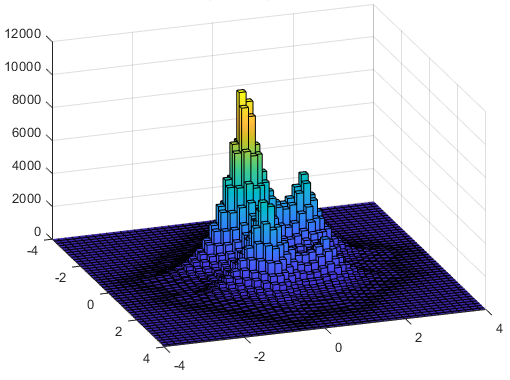
\includegraphics[width=1\linewidth]{hist3D}
	\caption{Histogram of the two-dimensional data generated from mixture of multivariate GGD.}
	\label{fig}
\end{figure}

\begin{figure}[H]
	\centering
	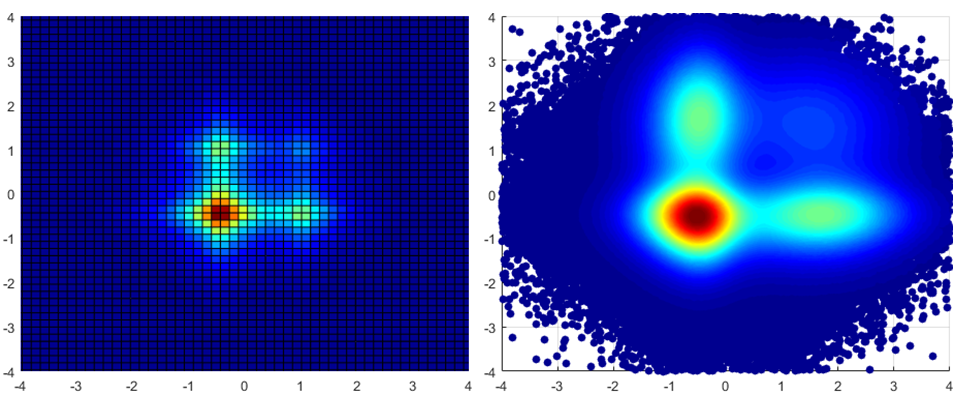
\includegraphics[width=1\linewidth]{ContourMatching}
	\caption{Contour plot of the two-dimensional data and its approximated PDF using the maximum entropy principle. Left: generated from mixture of multivariate GGD. Right: computed by the M-EMK.}
	\label{fig:mesh1}
\end{figure}

\begin{figure}[H]
	\centering
	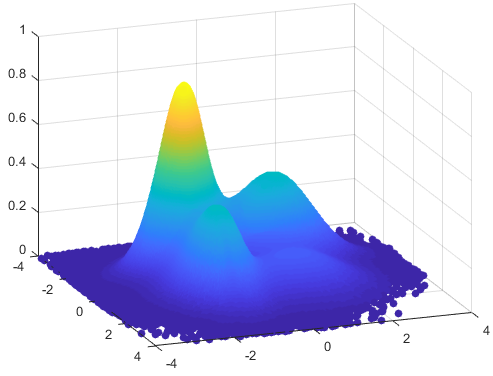
\includegraphics[width=1\linewidth]{pdf3D}
	\caption{Approximated PDF using the maximum entropy principle computed by the M-EMK.}
	\label{fig:mesh1}
\end{figure}

In figure 4, we show the density estimate using only global restrictions, as we can see, its performance is undesirable. Therefore, the local information obtained by using Gausian Kernels as a local constraint is very important for the effectiveness of M-EMK.
	
\begin{figure}[H]
	\centering
	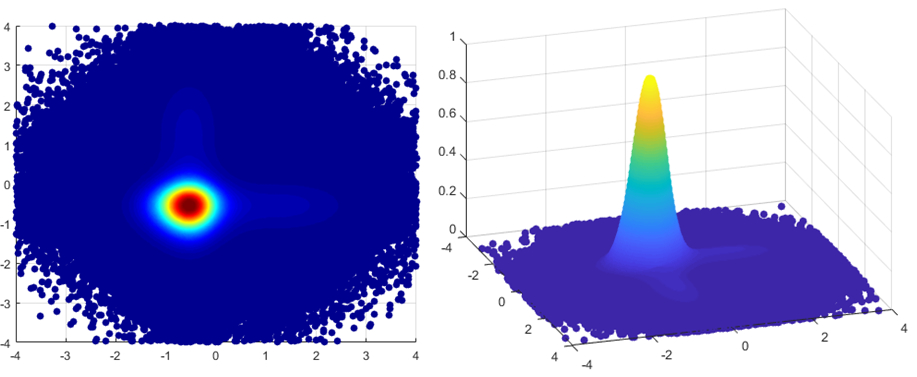
\includegraphics[width=1\linewidth]{OnlyGlobalConstMatching}
	\caption{Approximated PDF using only global constraints computed by the M-EMK.}
	\label{fig:mesh1}
\end{figure}


From equation (6) which represents the  cost function, we show in Fig. 6 the rapid convergence of M-EMK with respect to each iteration.
\begin{figure}[H]
	\centering
	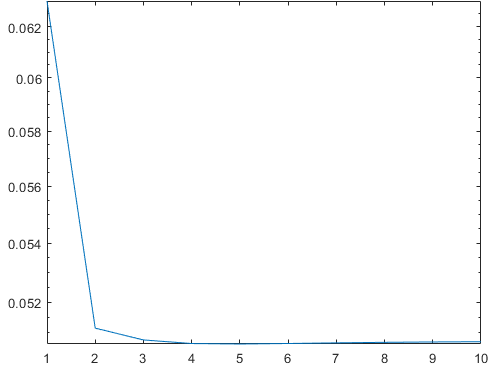
\includegraphics[width=0.8\linewidth]{CostFunction}
	\caption{Cost function with respect to each iteration.}
	\label{fig:mesh1}
\end{figure}


\section{DISCUSSIONS}
\label{sec:conc}
In this paper, we introduce the M-EMK, a new multivariate PDF estimation technique using the maximum entropy principle. By jointly using global and local constraints functions, M-EMK enjoys a high level of flexibility while providing a simple exponential form for PDFs in general. We show by experiments that M-EMK yields a very effective density estimation in terms of matching with the histogram. (Should we add information about Future Works? IVA-EMK (Zois's Proposals) , GANs...)


	
\bibliographystyle{IEEEtran}	
\bibliography{refs}

	
	
	
\end{document}


